% Digital Logic Report Template
% Created: 2020-01-10, John Miller

%==========================================================
%=========== Document Setup  ==============================

% Formatting defined by class file
\documentclass[11pt]{article}

% ---- Document formatting ----
\usepackage[margin=1in]{geometry}	% Narrower margins
\usepackage{booktabs}				% Nice formatting of tables
\usepackage{graphicx}				% Ability to include graphics
\usepackage[section]{placeins}  % Stops floats from happening

%\setlength\parindent{0pt}	% Do not indent first line of paragraphs 
\usepackage[parfill]{parskip}		% Line space b/w paragraphs
%	parfill option prevents last line of pgrph from being fully justified

% Parskip package adds too much space around titles, fix with this
\RequirePackage{titlesec}
\titlespacing\section{0pt}{8pt plus 4pt minus 2pt}{3pt plus 2pt minus 2pt}
\titlespacing\subsection{0pt}{4pt plus 4pt minus 2pt}{-2pt plus 2pt minus 2pt}
\titlespacing\subsubsection{0pt}{2pt plus 4pt minus 2pt}{-6pt plus 2pt minus 2pt}

% ---- Hyperlinks ----
\usepackage[colorlinks=true,urlcolor=blue]{hyperref}	% For URL's. Automatically links internal references.

% ---- Code listings ----
\usepackage{listings} 					% Nice code layout and inclusion
\usepackage[usenames,dvipsnames]{xcolor}	% Colors (needs to be defined before using colors)

% Define custom colors for listings
\definecolor{listinggray}{gray}{0.98}		% Listings background color
\definecolor{rulegray}{gray}{0.7}			% Listings rule/frame color

% Style for Verilog
\lstdefinestyle{Verilog}{
	language=Verilog,					% Verilog
	backgroundcolor=\color{listinggray},	% light gray background
	rulecolor=\color{blue}, 			% blue frame lines
	frame=tb,							% lines above & below
	linewidth=\columnwidth, 			% set line width
	basicstyle=\small\ttfamily,	% basic font style that is used for the code	
	breaklines=true, 					% allow breaking across columns/pages
	tabsize=3,							% set tab size
	commentstyle=\color{gray},	% comments in italic 
	stringstyle=\upshape,				% strings are printed in normal font
	showspaces=false,					% don't underscore spaces
}

% How to use: \Verilog[listing_options]{file}
\newcommand{\Verilog}[2][]{%
	\lstinputlisting[style=Verilog,#1]{#2}
}




%======================================================
%=========== Body  ====================================
\begin{document}

\title{ELC 2137 Lab \#\#: Lab Title}
\author{Put your name(s) here}

\maketitle


\section*{Summary}

The goal of this lab was to set up a circuit that displayed an 8-bit number on two 7-segment displays. In order to do this I need to create a multiplexer, a seven-segment decoder, a seven segement display (sseg1), and a wrapper. The multiplexer is used to switch between the digits of the display. When the switch is on, the number/letter will be displayed in the second colulmn (from the right) of the screen on the board and when the switch is off, the number/letter will be displyed in the first column (from the right) of the screen on the board. After I put together the multiplexer, I created a test bench to test it. The next design that I put together was the seven-segment decoder. The decoder takes in a four bit binary number and converts it to a 7-bit binary number. To make sure that the decoder worked, I created a test bench. Next, I created the 7-segment display (sseg1) which connected the decoder to the multiplexer. Again, I created one last test bench to make sure that they were properly connected. To clean up the code and make it more organized, I created a wrapper. The wrapper encompasses the sseg1 and connnects some of the wires. The wrapper connected the sw's, an's, dp's, and seg's together. Now I am able to program my board and see if it works. Once I connected my board I tested all of the values to see if it worked. Then I changed switch 15 to on and tested the values again. All of my results were correct. 


\section*{Q\&A}

1. How many wires are connected to the 7-segment display? \newline
There are 4 wires connected to the 7-segment display. There is 1 input and 3 outputs. \newline


2. If the segements were not all connected together, how many wires would there have to be? \newline
There would be 21 wires connected to the 7-segment display. \newline

3. Why do we prefer the current method vs. separating all of the segments? \newline
The current method is much simpler and much cleaner. The current method helps organized the circuit and make it more readable for the creator and for someone who is looking at your code. It will help in the future when you or someone else looks back on your code to see what you did. Instead of taking the time to firgure out where all 21 wires go, you can quickly see where the 4 groups of wires go. \newline


\section*{Results}

\begin{table}[h]\centering
	\begin{tabular}{cc}
		sel = 0 & sel = 1 \\
		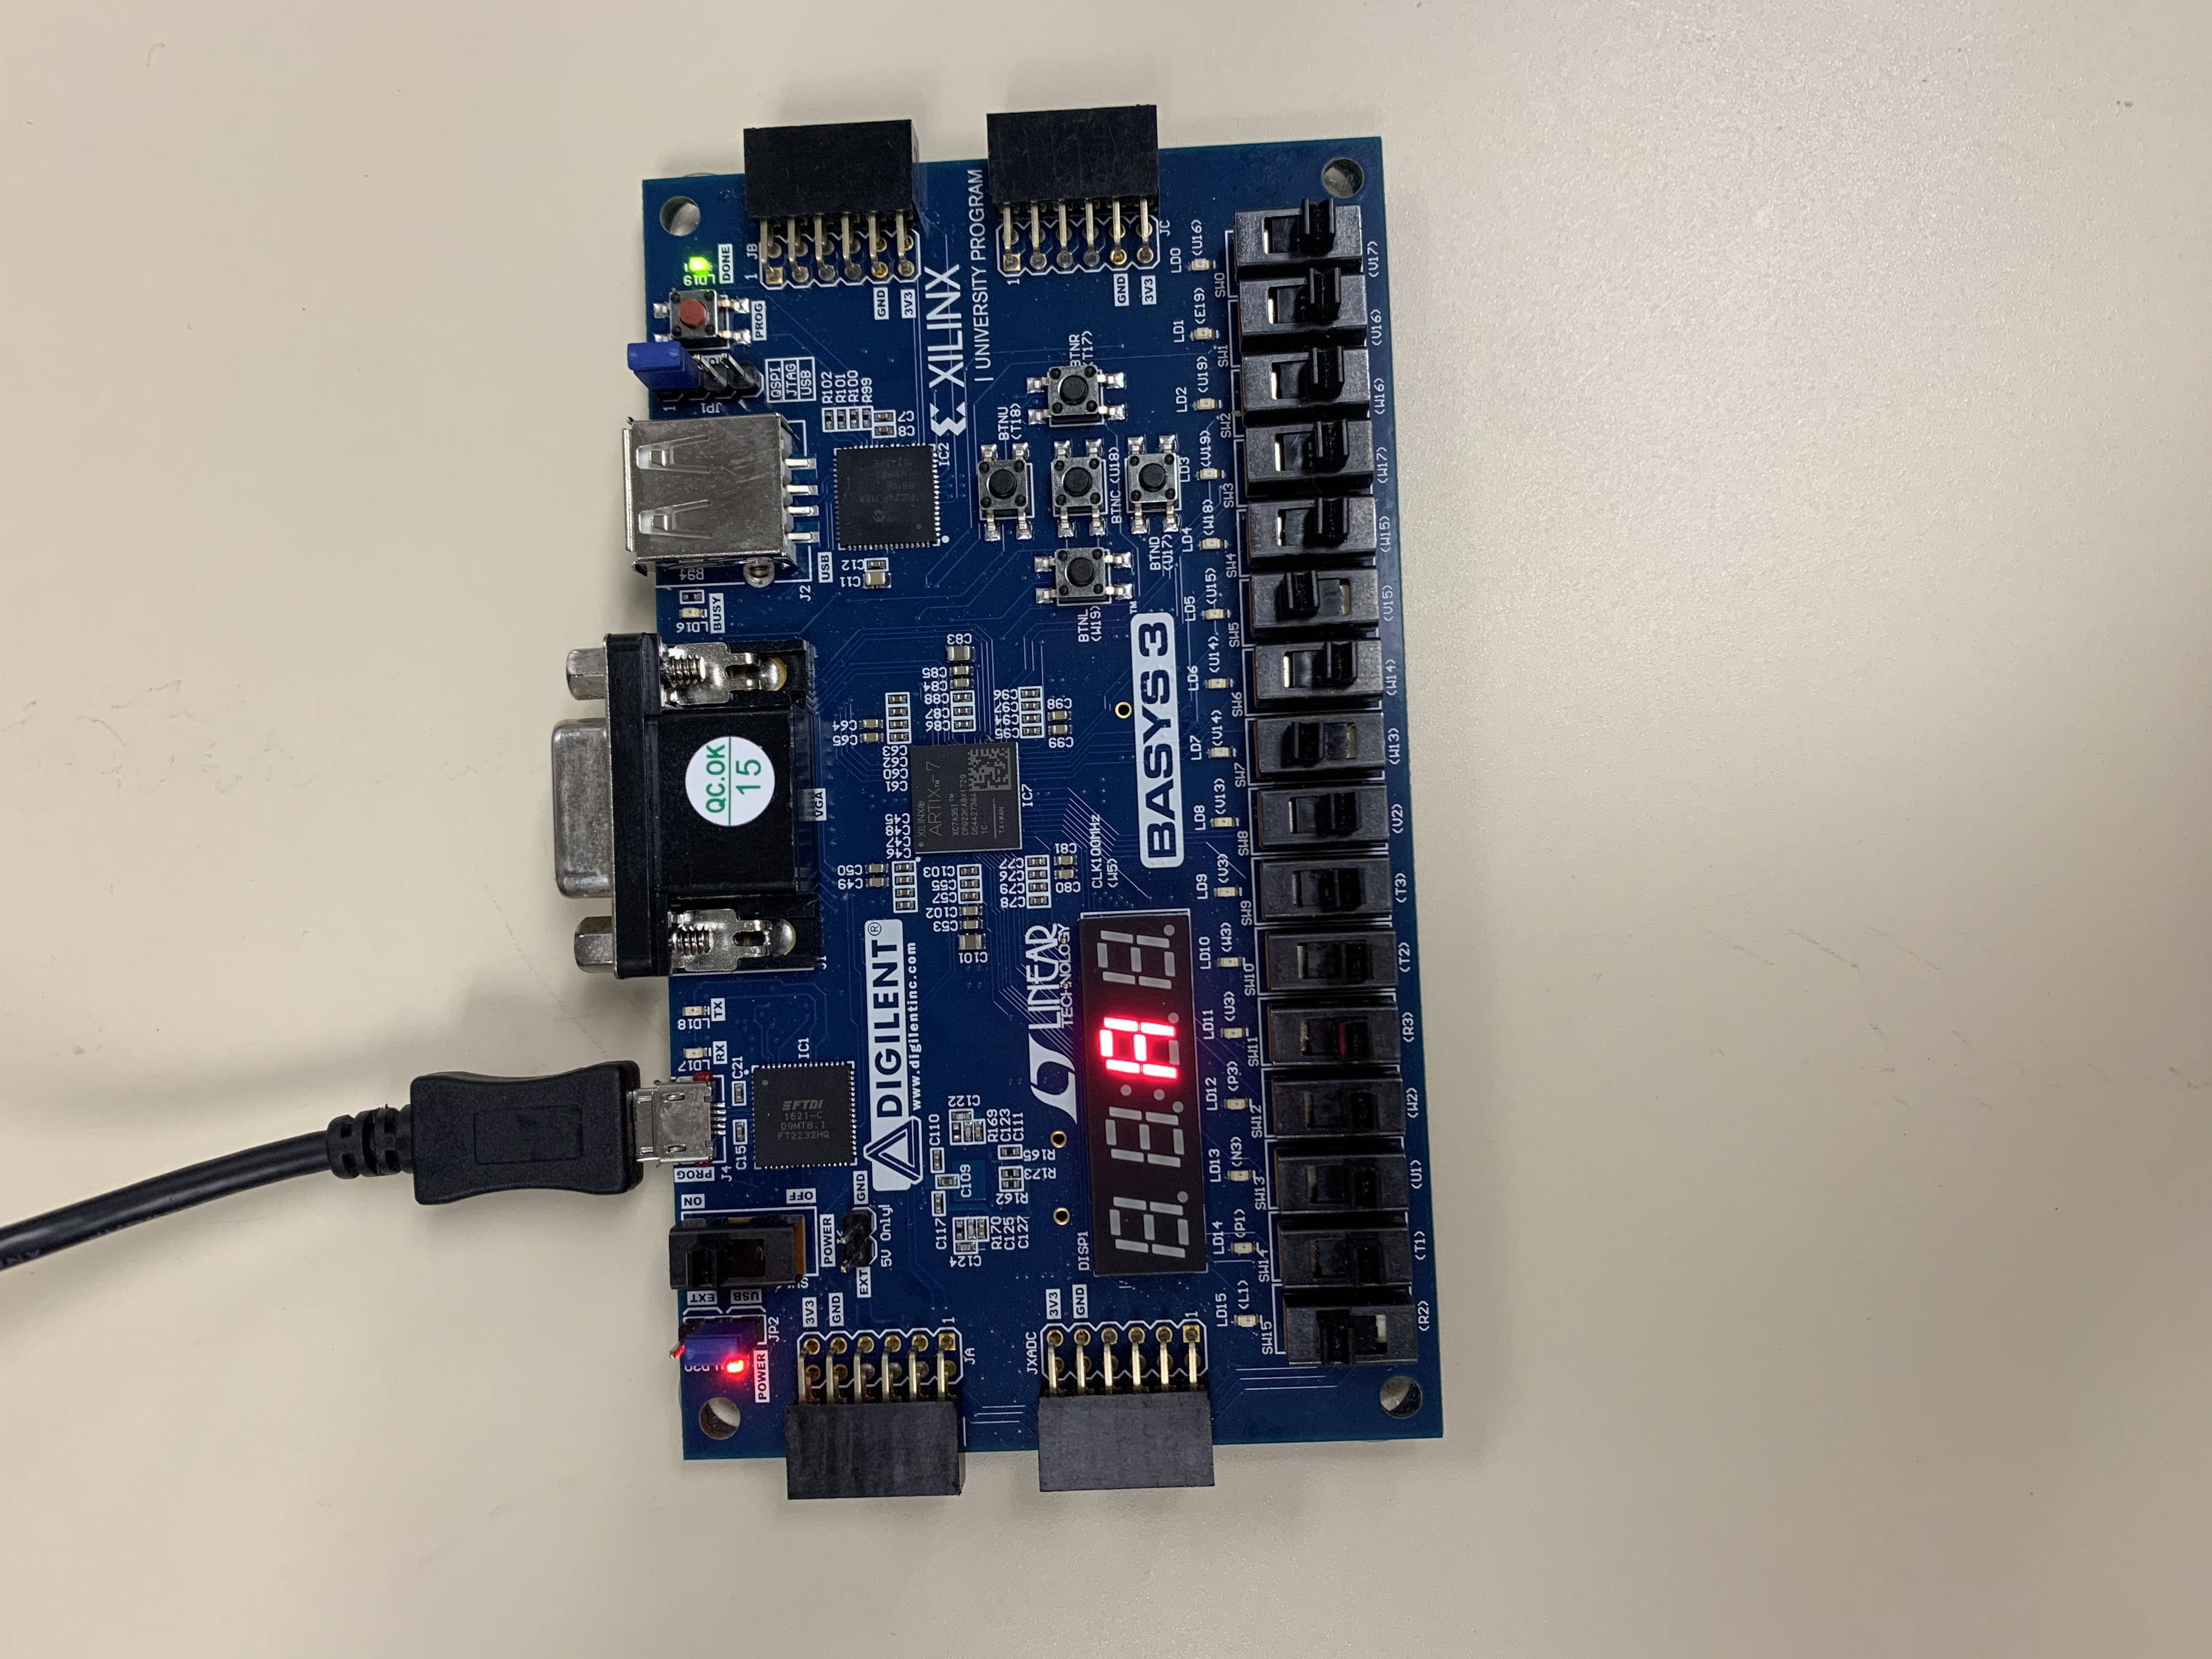
\includegraphics [width=0.5\textwidth,trim=0 0 0 0, clip, angle = 270]{Basys3_pic0} &
		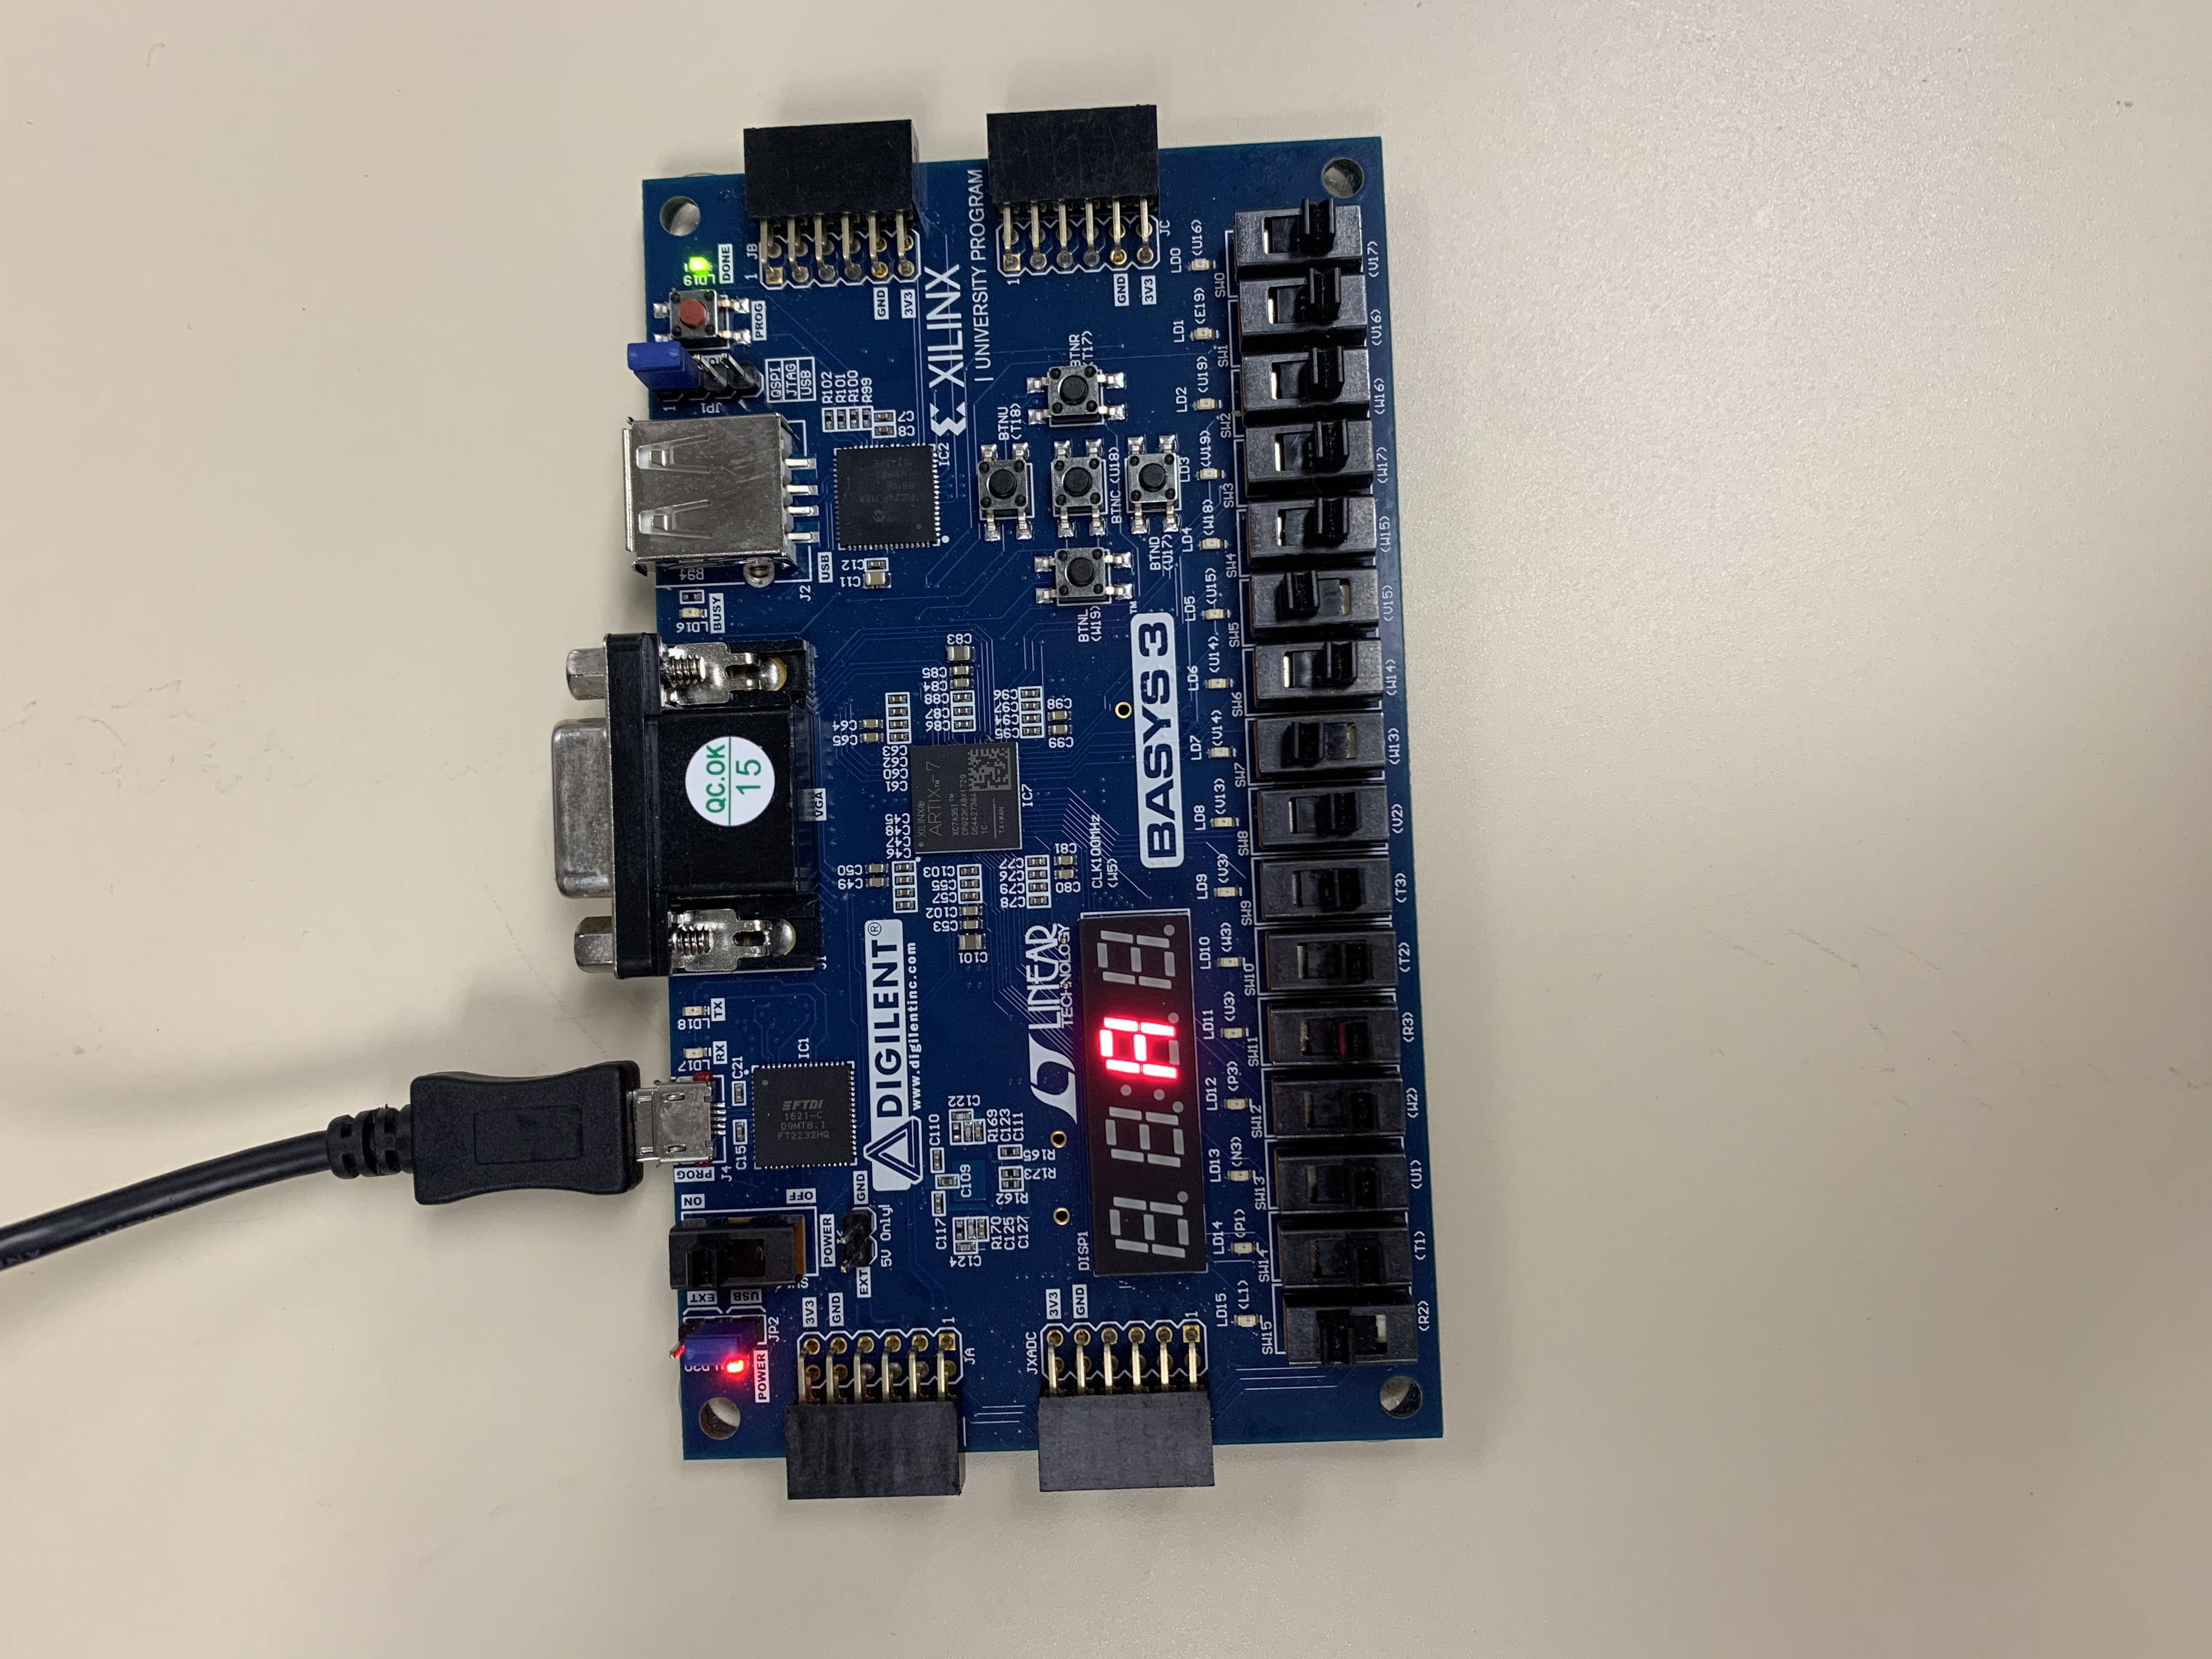
\includegraphics [width=0.5\textwidth,trim=0 0 0 0, clip, angle = 270]{Basys3_pic1} \\
	\end{tabular}
	\caption{Board Pictures}
	\label{fig:sim_with_table}
\end{table}




\section*{Code}




\end{document}
